% One-row main-text figure (2026-09-24): RL-Hammer (a) Llama (b) Qwen + (c) train-time ablation. Generated by
% paper/plot_rlhammer_ablation.py from the same data as fig_rlhammer.pdf and fig_ablation_v2.pdf. Replaces both figure
% environments in Sections 5.3 and 5.5.1; label fig:rlhammer is kept, fig:train_time_ablation refs become fig:rlhammer(c).

\begin{figure}[t]
  \centering
  \vspace{-0.1in}
  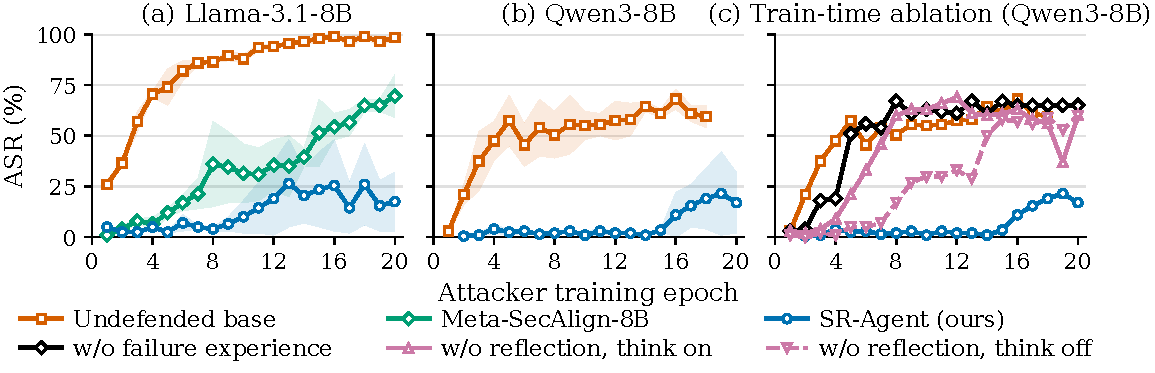
\includegraphics[width=\linewidth]{fig_rlhammer_ablation.pdf}
  \vspace{-0.2in}
  \caption{\textbf{Attack success rate over attacker training epochs under the RL-Hammer adaptive attack}, for
  (a) Llama-3.1-8B, (b) Qwen3-8B, and (c) the train-time ablation of self-reflection on Qwen3-8B
  (Section~\ref{sec:train_time_ablation}). In (a) and (b) each curve is the mean of two independent attacker runs
  against that target and the shaded band spans the two runs; endpoint statistics are reported in
  Tables~\ref{tab:rlhammer} and~\ref{tab:train_time_ablation}. Lower is better.}
  \vspace{-0.1in}
  \label{fig:rlhammer}
\end{figure}
